\documentclass{standalone}
\usepackage{tikz}
\usetikzlibrary{patterns, positioning}
\usepackage[sfdefault]{ClearSans} %% option 'sfdefault' activates Clear Sans as the default text font
\usepackage[T1]{fontenc}

\begin{document}
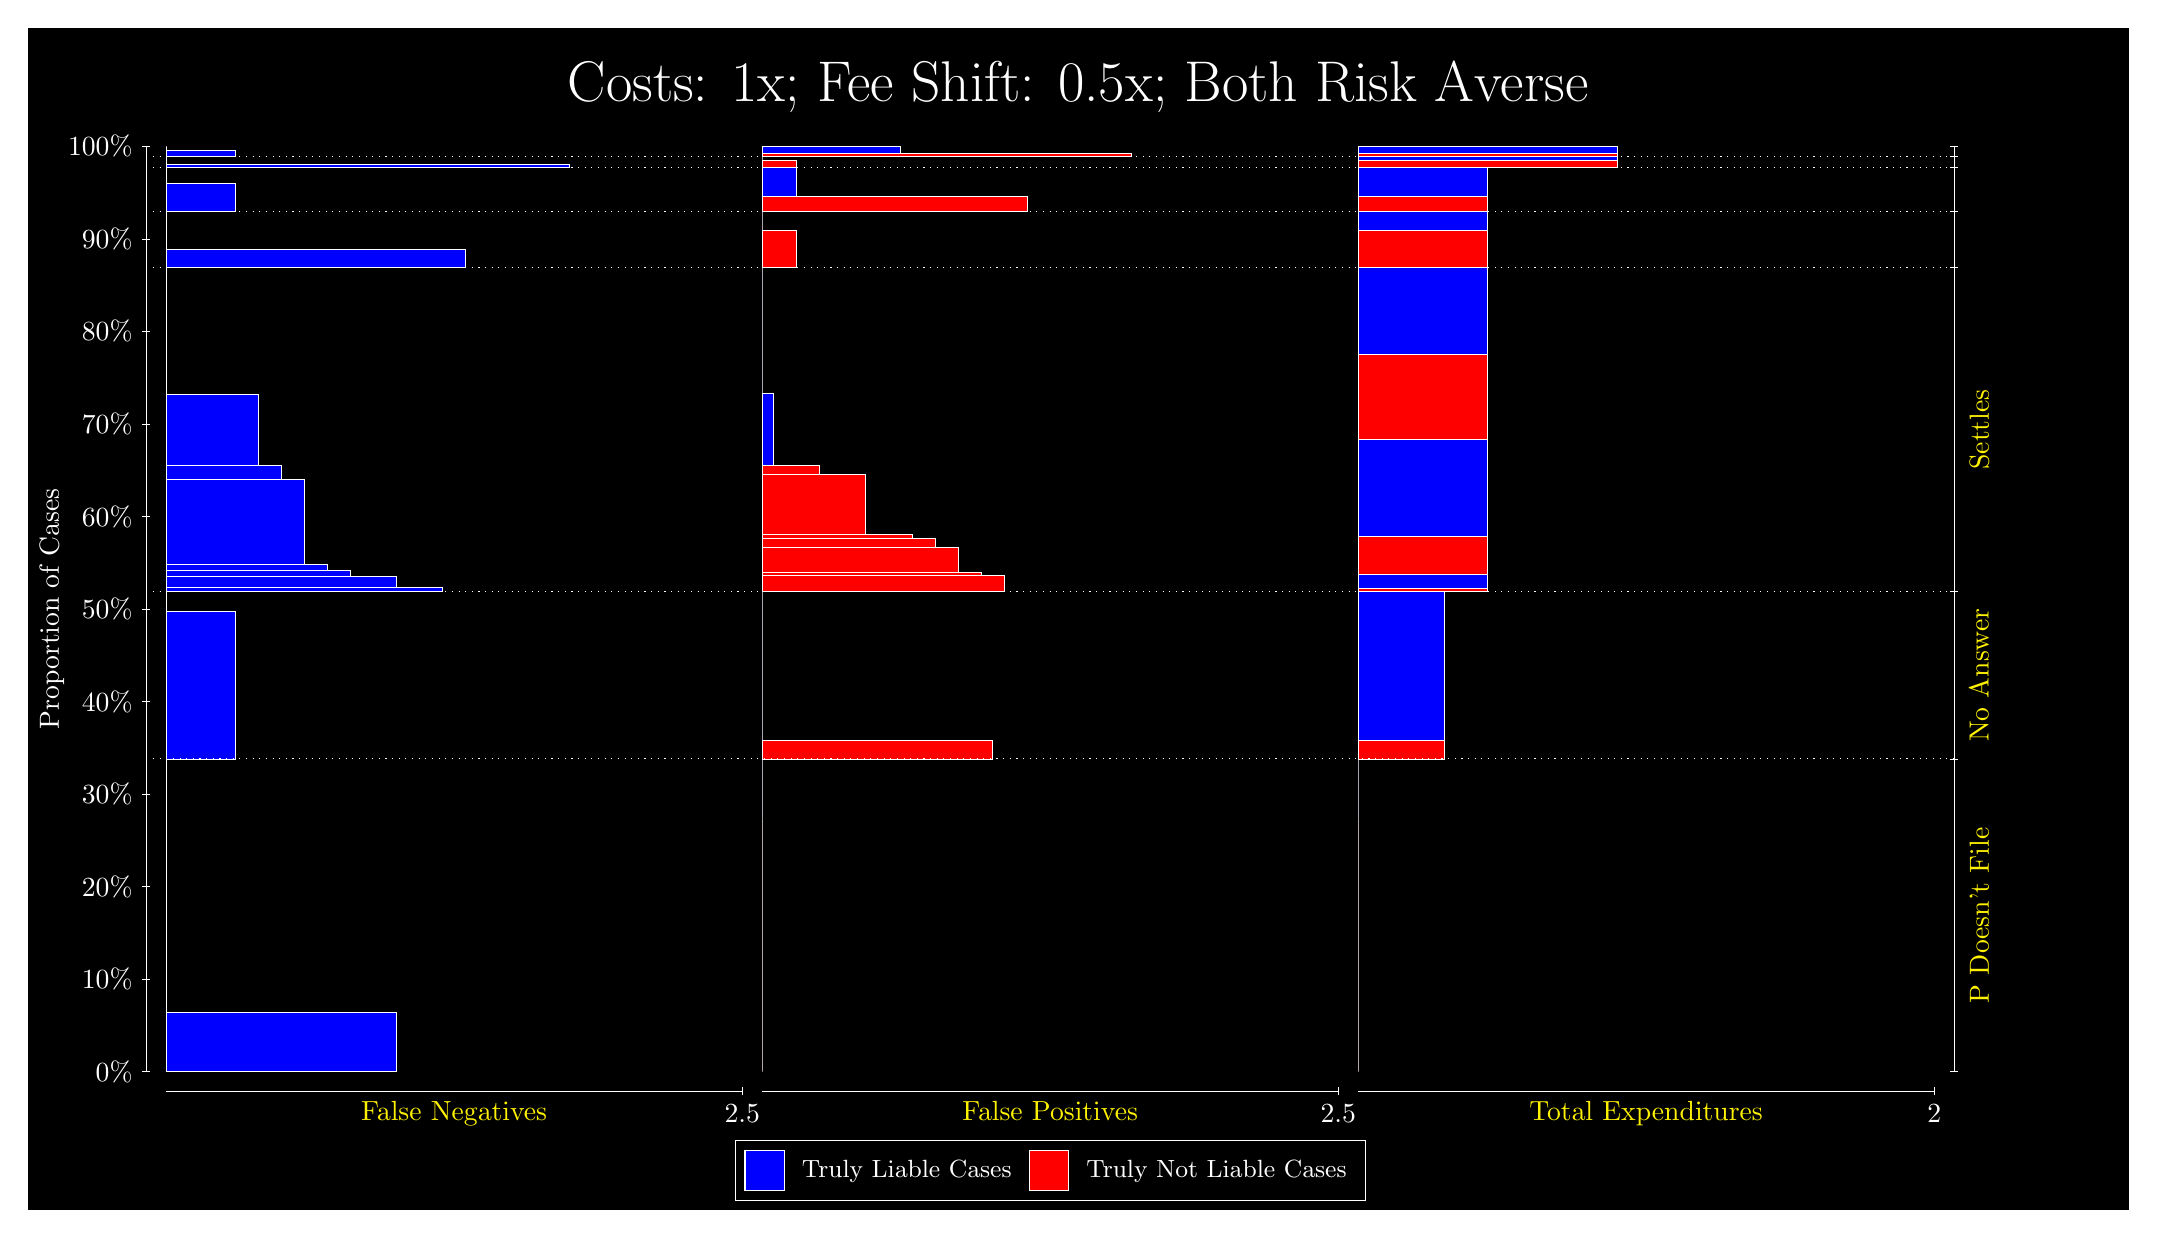
\begin{tikzpicture}
\draw[fill=black] (0,0) rectangle (26.667,15);
\draw[text=white] (0,13.5) rectangle (26.667,15) node[midway] {\huge Costs: 1x; Fee Shift: 0.5x; Both Risk Averse};
\draw[white, very thin] (1.5,1.75) -- (1.5,13.5);
\node[rotate=90, text=white, anchor=center] at (0.3, 7.625) {Proportion of Cases};
\draw[white, very thin] (1.45,1.75) -- (1.55,1.75);
\node[text=white, anchor=east] at (1.45, 1.75) {0\%};
\draw[white, very thin] (1.45,2.925) -- (1.55,2.925);
\node[text=white, anchor=east] at (1.45, 2.925) {10\%};
\draw[white, very thin] (1.45,4.1) -- (1.55,4.1);
\node[text=white, anchor=east] at (1.45, 4.1) {20\%};
\draw[white, very thin] (1.45,5.275) -- (1.55,5.275);
\node[text=white, anchor=east] at (1.45, 5.275) {30\%};
\draw[white, very thin] (1.45,6.45) -- (1.55,6.45);
\node[text=white, anchor=east] at (1.45, 6.45) {40\%};
\draw[white, very thin] (1.45,7.625) -- (1.55,7.625);
\node[text=white, anchor=east] at (1.45, 7.625) {50\%};
\draw[white, very thin] (1.45,8.8) -- (1.55,8.8);
\node[text=white, anchor=east] at (1.45, 8.8) {60\%};
\draw[white, very thin] (1.45,9.975) -- (1.55,9.975);
\node[text=white, anchor=east] at (1.45, 9.975) {70\%};
\draw[white, very thin] (1.45,11.15) -- (1.55,11.15);
\node[text=white, anchor=east] at (1.45, 11.15) {80\%};
\draw[white, very thin] (1.45,12.325) -- (1.55,12.325);
\node[text=white, anchor=east] at (1.45, 12.325) {90\%};
\draw[white, very thin] (1.45,13.5) -- (1.55,13.5);
\node[text=white, anchor=east] at (1.45, 13.5) {100\%};

\draw[white, very thin] (24.457,1.75) -- (24.457,13.5);
\draw[white, very thin] (24.407,1.75) -- (24.507,1.75);
\node[anchor=west] at (24.407, 1.75) {};
\draw[white, very thin] (24.407,5.72) -- (24.507,5.72);
\node[anchor=west] at (24.407, 5.72) {};
\draw[white, very thin] (24.407,7.844) -- (24.507,7.844);
\node[anchor=west] at (24.407, 7.844) {};
\draw[white, very thin] (24.407,11.961) -- (24.507,11.961);
\node[anchor=west] at (24.407, 11.961) {};
\draw[white, very thin] (24.407,12.67) -- (24.507,12.67);
\node[anchor=west] at (24.407, 12.67) {};
\draw[white, very thin] (24.407,13.228) -- (24.507,13.228);
\node[anchor=west] at (24.407, 13.228) {};
\draw[white, very thin] (24.407,13.368) -- (24.507,13.368);
\node[anchor=west] at (24.407, 13.368) {};
\draw[white, very thin] (24.407,13.5) -- (24.507,13.5);
\node[anchor=west] at (24.407, 13.5) {};

\draw[white, very thin, fill=blue] (1.75,1.75) rectangle (4.6775,2.5069);
\draw[white, very thin, fill=red] (1.75,2.5069) rectangle (1.75,5.72);
\draw[white, very thin, fill=blue] (1.75,5.72) rectangle (2.6283,7.6007);
\draw[white, very thin, fill=red] (1.75,7.6007) rectangle (1.75,7.844);
\draw[white, very thin, fill=blue] (1.75,7.844) rectangle (5.2631,7.8951);
\draw[white, very thin, fill=blue] (1.75,7.8951) rectangle (4.6775,8.0377);
\draw[white, very thin, fill=blue] (1.75,8.0377) rectangle (4.3848,8.0417);
\draw[white, very thin, fill=blue] (1.75,8.0417) rectangle (4.092,8.1104);
\draw[white, very thin, fill=blue] (1.75,8.1104) rectangle (3.7993,8.1962);
\draw[white, very thin, fill=blue] (1.75,8.1962) rectangle (3.5065,9.2711);
\draw[white, very thin, fill=blue] (1.75,9.2711) rectangle (3.2138,9.4461);
\draw[white, very thin, fill=blue] (1.75,9.4461) rectangle (2.921,10.353);
\draw[white, very thin, fill=red] (1.75,10.353) rectangle (1.75,11.961);
\draw[white, very thin, fill=blue] (1.75,11.961) rectangle (5.5558,12.198);
\draw[white, very thin, fill=red] (1.75,12.198) rectangle (1.75,12.67);
\draw[white, very thin, fill=blue] (1.75,12.67) rectangle (2.6283,13.029);
\draw[white, very thin, fill=red] (1.75,13.029) rectangle (1.75,13.228);
\draw[white, very thin, fill=blue] (1.75,13.228) rectangle (6.8732,13.272);
\draw[white, very thin, fill=red] (1.75,13.272) rectangle (1.75,13.368);
\draw[white, very thin, fill=blue] (1.75,13.368) rectangle (2.6283,13.456);
\draw[white, very thin, fill=red] (1.75,13.456) rectangle (1.75,13.5);
\draw[white, very thin, fill=red] (9.3189,1.75) rectangle (9.3189,4.963);
\draw[white, very thin, fill=blue] (9.3189,4.963) rectangle (9.3189,5.72);
\draw[white, very thin, fill=red] (9.3189,5.72) rectangle (12.246,5.9632);
\draw[white, very thin, fill=blue] (9.3189,5.9632) rectangle (9.3189,7.844);
\draw[white, very thin, fill=red] (9.3189,7.844) rectangle (12.393,8.049);
\draw[white, very thin, fill=red] (9.3189,8.049) rectangle (12.1,8.0934);
\draw[white, very thin, fill=red] (9.3189,8.0934) rectangle (11.807,8.4107);
\draw[white, very thin, fill=red] (9.3189,8.4107) rectangle (11.515,8.5172);
\draw[white, very thin, fill=red] (9.3189,8.5172) rectangle (11.222,8.5747);
\draw[white, very thin, fill=red] (9.3189,8.5747) rectangle (10.929,8.5786);
\draw[white, very thin, fill=red] (9.3189,8.5786) rectangle (10.636,9.3381);
\draw[white, very thin, fill=red] (9.3189,9.3381) rectangle (10.051,9.4522);
\draw[white, very thin, fill=blue] (9.3189,9.4522) rectangle (9.4652,10.359);
\draw[white, very thin, fill=blue] (9.3189,10.359) rectangle (9.3189,11.961);
\draw[white, very thin, fill=red] (9.3189,11.961) rectangle (9.758,12.433);
\draw[white, very thin, fill=blue] (9.3189,12.433) rectangle (9.3189,12.67);
\draw[white, very thin, fill=red] (9.3189,12.67) rectangle (12.686,12.869);
\draw[white, very thin, fill=blue] (9.3189,12.869) rectangle (9.758,13.228);
\draw[white, very thin, fill=red] (9.3189,13.228) rectangle (9.758,13.324);
\draw[white, very thin, fill=blue] (9.3189,13.324) rectangle (9.3189,13.368);
\draw[white, very thin, fill=red] (9.3189,13.368) rectangle (14.003,13.411);
\draw[white, very thin, fill=blue] (9.3189,13.411) rectangle (11.075,13.5);
\draw[white, very thin, fill=red] (16.888,1.75) rectangle (16.888,4.963);
\draw[white, very thin, fill=blue] (16.888,4.963) rectangle (16.888,5.72);
\draw[white, very thin, fill=red] (16.888,5.72) rectangle (17.986,5.9632);
\draw[white, very thin, fill=blue] (16.888,5.9632) rectangle (17.986,7.844);
\draw[white, very thin, fill=red] (16.888,7.844) rectangle (18.534,7.8885);
\draw[white, very thin, fill=blue] (16.888,7.8885) rectangle (18.534,8.0634);
\draw[white, very thin, fill=red] (16.888,8.0634) rectangle (18.534,8.5446);
\draw[white, very thin, fill=blue] (16.888,8.5446) rectangle (18.534,9.7741);
\draw[white, very thin, fill=red] (16.888,9.7741) rectangle (18.534,10.857);
\draw[white, very thin, fill=blue] (16.888,10.857) rectangle (18.534,11.961);
\draw[white, very thin, fill=red] (16.888,11.961) rectangle (18.534,12.433);
\draw[white, very thin, fill=blue] (16.888,12.433) rectangle (18.534,12.67);
\draw[white, very thin, fill=red] (16.888,12.67) rectangle (18.534,12.869);
\draw[white, very thin, fill=blue] (16.888,12.869) rectangle (18.534,13.228);
\draw[white, very thin, fill=red] (16.888,13.228) rectangle (20.181,13.324);
\draw[white, very thin, fill=blue] (16.888,13.324) rectangle (20.181,13.368);
\draw[white, very thin, fill=red] (16.888,13.368) rectangle (20.181,13.411);
\draw[white, very thin, fill=blue] (16.888,13.411) rectangle (20.181,13.5);
\draw[white, dotted] (1.5,5.72) -- (24.457,5.72);
\draw[white, dotted] (1.5,7.844) -- (24.457,7.844);
\draw[white, dotted] (1.5,11.961) -- (24.457,11.961);
\draw[white, dotted] (1.5,12.67) -- (24.457,12.67);
\draw[white, dotted] (1.5,13.228) -- (24.457,13.228);
\draw[white, dotted] (1.5,13.368) -- (24.457,13.368);
\draw[white, very thin] (1.75,1.5) -- (9.0689,1.5);
\node[text=yellow, anchor=north] at (5.4094, 1.5) {False Negatives};
\draw[white, very thin] (9.0689,1.45) -- (9.0689,1.55);
\node[text=white, anchor=north] at (9.0689, 1.45) {2.5};

\draw[white, very thin] (9.3189,1.5) -- (16.638,1.5);
\node[text=yellow, anchor=north] at (12.978, 1.5) {False Positives};
\draw[white, very thin] (16.638,1.45) -- (16.638,1.55);
\node[text=white, anchor=north] at (16.638, 1.45) {2.5};

\draw[white, very thin] (16.888,1.5) -- (24.207,1.5);
\node[text=yellow, anchor=north] at (20.547, 1.5) {Total Expenditures};
\draw[white, very thin] (24.207,1.45) -- (24.207,1.55);
\node[text=white, anchor=north] at (24.207, 1.45) {2};

\node[text=yellow, centered, rotate=90] at (24.777, 3.735) {P Doesn't File};
\node[text=yellow, centered, rotate=90] at (24.777, 6.782) {No Answer};
\node[text=yellow, centered, rotate=90] at (24.777, 9.9025) {Settles};





\draw (12.978300999999998,1.5) node[draw=none] (baseCoordinate) {};
\begin{scope}[align=center]
        \matrix[scale=0.5, draw=white, below=0.5cm of baseCoordinate, nodes={draw}, column sep=0.1cm]{
            \node[rectangle, draw, minimum width=0.5cm, minimum height=0.5cm, fill=blue] {}; &
            \node[draw=none, font=\small, text=white] (B) {Truly Liable Cases}; &
            \node[rectangle, draw, minimum width=0.5cm, minimum height=0.5cm, fill=red] {}; &
            \node[draw=none, font=\small, text=white] (B) {Truly Not Liable Cases}; \\
            };
\end{scope}

\end{tikzpicture}
\end{document}